\documentclass[11pt, twocolumn]{report}
\usepackage[a4paper, hmargin={2.8cm, 2.8cm}, vmargin={2.5cm, 2.5cm}]{geometry}
%\usepackage[T1]{fontenc}
\usepackage[utf8]{inputenc}
\usepackage{eso-pic} % \AddToShipoutPicture
\usepackage{graphicx} % \includegraphics
\usepackage[english]{babel}
\usepackage{tcolorbox}
\usepackage{multicol}
\usepackage{amssymb}
\usepackage{amsmath}
\usepackage{fancyhdr}
\usepackage{fancyvrb}
\usepackage{geometry}
\usepackage{listings}
\usepackage[hyphens]{url}
\usepackage{breakurl}
\usepackage{cite}
\usepackage{color}
\usepackage{array}
\usepackage{multicol}
\usepackage[toc,page]{appendix}
\usepackage[breaklinks=true]{hyperref}
\usepackage{float}
\usepackage{xcolor}
\usepackage{tablefootnote}
\usepackage{footnote}
\usepackage{lipsum}
\usepackage{tocloft}


%%% Macros
% easier figure
% usage: \pic{width}{image}{caption}{label} 
\newcommand\pic[4]{% these comment signs will prevent the introduction of spurious spaces
  \begin{figure}[h!]
  \centering
  \includegraphics[width=#1\textwidth]{#2}
  \caption{#3}
  \label{#4}
  \end{figure}
}




\newcolumntype{C}[1]{>{\centering\let\newline\\\arraybackslash\hspace{0pt}}m{#1}}
\setlength{\columnsep}{1cm}


\author{
  Meznik, Jan\\
  \texttt{pzj895@alumni.ku.dk}\\
  \texttt{jan@meznik.dk}
  \and
  Jacobi, Mark Jan\\
  \texttt{dcz738@alumni.ku.dk}
}

\title{
	\vspace{3cm}
	\huge{TCP/IP in hardware using SME}\\
		\vspace{0.5cm}
	\Large{Write something clever here}
}



% Header
\pagestyle{fancy}


\iffalse
\fancyhf{}
%\fancyhead[L]{}
%\fancyhead[R]{}
%\fancyhead[C]{}
%\fancyfoot[C]{Center \leftmark}
\fi

\lhead{University of Copenhagen}
%\chead{}
\rhead{TCP/IP in SME}


\begin{document}
\onecolumn


%%%%% KU HEADER %%%%%%%%%%%%%%%%%%%%%%%
\AddToShipoutPicture*{\put(0,0){\includegraphics*[viewport=0 0 700 600]{include/natbio-farve}}}
\AddToShipoutPicture*{\put(0,602){\includegraphics*[viewport=0 600 700 1600]{include/natbio-farve}}}
\AddToShipoutPicture*{\put(0,0){\includegraphics*{include/nat-en}}}
\clearpage
\maketitle
\pagenumbering{roman}
\thispagestyle{empty}
\newpage
%%%%%%%%%%%%%%%%%%%%%%%%%%%%%%%%%%%%%%%


%\begin{abstract}
\thispagestyle{empty}
%In this thesis, we design and implement a networking protocol stack in hardware
using the Synchronous Message Exchange model -- a new framework intended to
help model hardware descriptions.  The final pipelined design boasts with
a decentralized memory model, with model division easily extensible and
modifiable, closely ressembling that of the architecture of the Internet
Protocol Suite.

Initial tests performed on the simulated system with real captured network
traffic suggests stability, promising protocol compliance, and an acceptable, but
theoretical, performance. Numerous suggestions are discussed to improve the performance,
such as widening the bus-widths or replicating the stack itself to multiply the
raw throughput.

Due to some trivial bugs and other minor missing features in the SME framework,
the system could not be brought to the target FPGA hardware. However, we are
optimistic that considerable performance is achieveable with the current design,
as well as great flexibility, extensibility and modularity of the system.



\newpage
%\end{abstract}


%\section*{Overview}
%\input{overview/overview.tex}

\newpage

% \section*{Preface}
% \input{preface/preface.tex}
\newpage
\twocolumn

\thispagestyle{empty}
\tableofcontents
\renewcommand{\cftchapleader}{\cftdotfill{\cftdotsep}} 
\renewcommand{\cftsecleader}{\cftdotfill{\cftdotsep}}
\onecolumn
\newpage
\twocolumn

\clearpage
\pagenumbering{arabic}
\setcounter{page}{1}

\markboth{Name}{Report}
\noindent

\chapter{Introduction}
% 1. general introduction
This thesis describes the design and implementation of an efficient, high-speed
TCP/IP network stack intended to run on custom hardware where performance, responsiveness,
and throughput is crucial.\\

% 2. Explanation of specific problem
As is the trend with modern automation, computerization, and mechanization, new
devices are steadily invented to handle this increasing demand for data and
control.
With the ever-increasing sophistication of machines generating immense amount
of information, the data needs to be transmitted to numerous other machines for
further processing, or even simply storage. The most common and the most convenient
way of linking multiple devices together is using the internet, and its underlying
protocols. However, the networking stack supplied with most major operating
systems, while heavily optimised, suffers from considerable penalties due to
complexities of a standard computer architecture. For example, heavy network
traffic utilizes the computers' internal busses, utilizes the memory, and spend
precious \gls{cpu} clock-cycles with polling and interrupts. This
prevents the machine from using these resources for actual computing tasks.\\
These issues have been identified and solved by hardware manufacturers by
adopting dedicated \gls{nic}, which would employ
various techniques to offload the processing. One such offloading technique is
called the \gls{toe}, which usually takes care of the essential
parts of networking involved -- the \gls{ip} and the \gls{tcp}\cite{TCP_offload_dumb_idea}.\\
Modern hardware manufacturers can produce NICs boasting network throughput
speeds as high as 100 Gigabits\cite{xilinx_100g_nic}. Unfortunately, these cards
are highly specialized for certain applications, and even though they provide
basic programmability, they are rarely suitable for rapid prototyping of
applications and other custom hardware devices. Furthermore, each NIC manufacturer
has a diverse set of hardware with varying interfaces, making it hard to
combine, swap and test these cards.
Licensed software solutions in the form of IP blocks exist as well
\cite{microtronix_ip_cores}\cite{avnet_ip_cores}. Unfortunately,
these blocks are usually distributed as black-boxes of \gls{vhdl}
code, which is hard to maintain, and even harder to debug and
extend\cite{opencores_mission}.  Additionally, these IP blocks or
"cores" are exceptionaly expensive for smaller design teams, making
it nearly impossible to prototype hardware designs with limited
funding\cite{opencores_mission}. Multiple networking IP cores exist gratis for
non-commercial use, but use for these is very limited by that nature.
Bying a licence for such IP cores is not an easy task either, as the
prices of the licenses are rarely listed on the vendor sites, and the
sales departments have to be contacted for a custom quotation. It is
also common to either require a lawyer to verify and sign the excessive
license agreements, or having to sign up for memberships of various
IP Licensing deals, such as the SignOnce IP Licensing program by
Xilinx\cite{xilinx_signonce}.\\

In this thesis, we bridge the gap between the blazingly-fast network offloading
devices and their more flexible and malleable software counterparts.\\
This networking stack is implemented in a fully self-contained fashion so that
it is completely independent of any other software running on the machine, while
utilizing the performance advantages gained from the lack of overhead in
conventional implementations.
The use of a high-level programming language in combination with the modern
\gls{sme} model makes the network stack a very versatile
implementation with ease of use, debugging, and even extension.


\section{Related work}
Networking is indeed desired in more and more applications and hardware devices.
As a consequence, there exist projects that bring the internet protocol suite to
the FPGA hardware. One such project is the Xilinx 10Gbps TCP/IP Stack,
implementing a full TCP/IP stack inside the FPGA. It supports \gls{tcp} and
\gls{udp} for data-transmission as well as auxiliary protocols, such as
\gls{ipv4}, \gls{icmp}, \gls{arp}, and \gls{dhcp}.
This network stack is able to maintain a stable connection of 10Gbps, and higher
speeds are easily reachable with better hardware\cite{sidler2015tcp}.\\
The network stack has been implemented in C++ using the Vivado High-Level
Synthesis compiler, generating the underlying \gls{rtl} model, greatly increasing
the programmer productivity.
To achieve performance in the \gls{hls} C++ language, special loop pipelining and
loop unrolling annotiations are used to transform loops from conventional
sequentially-executed loops to fully parallel loops\cite{xilinx_loop_unrolling}.
These annotations are not a part of the core C++ language, and they cannot be
added generated automatically without the risk of creating race conditions and
other bugs. As such, the loop unrolling has to be done by the programmer, and
the performance of the finished product relies solely on the ability of the
programmer to unroll and pipeline the loops efficiently and without errors.\\
The architecture of the Xilinx TCP/IP stack, seen on figure \ref{fig:fccm2015},
is very similar to the one described in the implementation chapter.
\ref{chap:implementation}.
\begin{figure}[h]
\centering
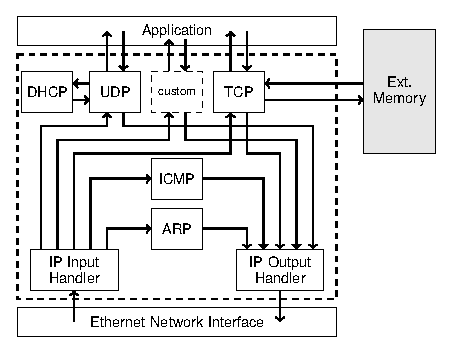
\includegraphics[scale=1]{introduction/fccm2015.eps}
\caption{The architecture of the Xilinx 10Gbps TCP/IP stack introduced in
\textit{Scalable 10Gbps TCP/IP Stack Architecture for Reconfigurable Hardware,
in FCCM’15}\cite{sidler2015tcp}.}
\label{fig:fccm2015}
\end{figure}



\chapter{Background}

In this chapter, we will introduce the basic concepts of the Internet Protocol
Suite, briefly describe its origin, semantics, and some of its protocols.
Furthermore, SME and the hardware it will run on will be introduced as a basis
for the implementation.


\section{Internet Protocol Suite (TCP/IP)}
Internet Protocol Suite, better known as simply TCP/IP, is a conceptual
model providing end-to-end communication between computers. It consists of
a collection of protocols specifying the communication between multiple
Internet systems\cite{RFC1122}.  The very early research and development
on what would later become the Internet Protocol Suite began in the late 1960s
by the Defense Advanced Research Project Agency (DARPA), and was being
adopted by DARPA, as well as the public, since 1983\cite{DARPA_internet}.
Although the Internet Protocol Suite predates the newer, arguably more
refined Open Systems Interconnection (OSI) model, TCP/IP still
remains the popular choice in modern systems.  As opposed to OSI 7-layer
model\cite{X.200}, the collection of protocols in TCP/IP are organized
into 4 abstraction layers, each related to their scope of networking
involved.

\subsection{Link Layer}
The link layer is the lowest, bottom-most layer in the Internet Protocol Suite.
Link layer addresses methods and protocols operating on the link that the host
is physically connected to\footnote{Wireless connections are also included
under this category.}. Contrary to the OSI model, this lowest layer in TCP/IP
does not regard the standards and protocols of the physical mediums used (the
pin layout, voltages, cable specifications etc.), making TCP/IP hardware-independent.
As a result, TCP/IP can in theory be implemented on virtually any hardware
configuration, emphasizing the flexibility of the model.

\subsection{Internet Layer}
The internet layer mainly concerns itself with sending data from the source
network to the destination network. This seemingly simple task requires multiple
functions from the layer:
\begin{itemize}
    \item Addressing and identification
    \item Packet routing
    \item \emph{Basic} transmit diagnostic information
    \item Carrying data for various upper layer protocols
\end{itemize}


\subsection{Transport Layer}
The transport layer establishes end-to-end data transfer between hosts.
Protocols in the transport layer can provide additional services to the user,
such as reliability, ordering, error- and flow-control, application addressing
(port numbers), error-checking, and so on.\\
While it is possible to bypass the protocols in this layer on most modern
network stacks, the protocols in the transport layer provide such essential
and useful services that it hardly ever makes sense to implement in the
application layer.\\
While there are numerous protocols defined in the Transport Layer, perhaps the
most well-known protocol in the stack is the Transmission Control Protocol (TCP).
Being one of the most used transport protocol for its reliability and congestion
control systems, it is rightly justified to refer to the whole Internet Protocol
Suite as simply "TCP/IP".


\subsection{Application Layer}
The application layer protocols are used by applications and services to
exchange information over the network. A few of the well-known application
layer protocols are the Hypertext Transfer Protocol (HTTP)\cite{RFC1945},
File Transfer Protocol (FTP)\cite{RFC0114}, and Simple Mail Transfer Protocol
(SMTP)\cite{RFC0788}.\\
This layer is usually implemented by the userspace applications themselves, and
therefore are not strictly required to actually run a TCP/IP network.



\section{Hardware}
The networking stack is intended to be flexible enough to run on just about any
configuration of hardware and software. However, this also means that it cannot
depend on any major external components, such as an existing memory, a processor,
or any form of operating system. Fundamentally, not only the software-part of the
networking stack has to be implemented, but the hardware needs to be defined
as well. This hardware should be self-contained enough to work well in combination
with any additional system, which the user incorporate for networking.\\
A wide variety of hardware types exist for such independent system, such as
Application-specific Integrated Circuit (ASIC), Complex Programmable Logic
Device (CPLD), Socket on a Chip (SoC), and Field-Programmable Gate Array (FPGA).
Each of these integrated circuits have their advantages and disadvantages; some
of them are re-programmable, some are cheap and disposable, and some are excellent
for general-purpose applications.\\
In this thesis, only FPGAs will be taken into consideration for its re-programmability,
its fairly low-cost, and the compatibility with SME code-generators.


\subsection{Field Programmable Gate Array (FPGA)}
Field Programmable Gate Arrays, or FPGA for short, are devices containing
integrated circuits (ICs) consisting of arrays of logic blocks.
These logic blocks can be programmed to form arbitrary logic circuit by simply
synthesizing a design and then loading it onto the board. This process alone
can save the manufacturer months by not having to fabricate a whole new IC. \\
FPGAs can be used for any computational tasks without the need of any additional
hardware. Usually, these devices are used for smaller, domain-specific tasks,
where the control over the hardware yields significant performance increases.
FPGAs are indeed very universal, and can be used in product-design, prototyping,
as well as in final products. Products like car driver assistance
systems\cite{xilinx_fpga_automotive}, audio decoders\cite{xilinx_fpga_audio},
or even internet search engines\cite{bing_search_fpga}  all utilize FPGAs to
increase the performance, lower the electrical bill, and  boost the development
potential.


\subsubsection{Technical specifications}
Field Programmable Gate Arrays consists of a vast number of ICs, which can
be reprogrammed at any time for a desired application or functionality\cite{ni_fpga},
making the devices very flexible and extensible, even after manufacturing.\\
These ICs are practically totally independent, and their logic within can be
programmed and combined in virtually any way with other ICs. This, however,
poses a problem, as signals do not propagate through circuitry, immediately, but
rather, they have a slight delay.
Sometimes, two events precede each other, while other times, events of distinct
timings must occur simultaneously.
Since the order of events is critical for correct and expected execution in
digital circuits, a digital clock is used to ensure everything runs in sync.
A clock in this context emits a series of pulses in a pre-determined and very
precise interval. These pulses are used to control the execution of various
elements in the circuitry.\\
When synthesizing to a FPGA, the compiler finds the longest code-path, it finds
the required circuitry to perform the calculation, and then it determines the
minimal required time for the signals to propagate through the path. In this
manner, the fastest possible clock can be found for that particular circuit.\footnote{
    Although many modern FPGAs consist of multiple regions which can have individual
    clock-rates. While it is a demanding task to propagate signals across these
    boundaries, a performance increases can be gained.
}
With innovations and steady improvements in modern FPGAs, the circuitries within
the devices can be clocked at higher than 500 MHz\cite{xilinx_fpga}.



\subsubsection{Programming an FPGA}
Unlike conventional processors with a very sequential nature, the logic blocks
in FPGAs are truly parallel in nature. Given the right programming, an FPGA can
allocate dedicated sections of the chip for each independent subtask, enabling
the circuitry to perform numerous independent calculations at once\cite{ni_fpga}.
Unfortunately, this universality of FPGAs comes at a cost to their performance.
Whereas conventional processors are heavily optimise based on the predetermined
circuitry, FPGAs programmers must ensure to utilize the parallel nature of the
device in order to secure best possible performance. Even worse, the FPGA must
be programmed in such a way that all paths in the electrical wiring can be
in any time-frame.\\
Due to this parallel nature of FPGAs, conventional programming languages are
next to impossible to use. To define the behavior of an FPGA, Hardware
Description Languages (HDL) are used. These programming languages are not easy
to learn without a good grasp of electrical engineering. Even with prior
programming knowledge, the unusual approach to concurrency in these languages
can be hard to understand for average developers.\\
To simplify the development process, most manufacturers offer predefined
circuits along their FPGAs. These predefined circuits are more commonly known
as Intellectual Property (IP) cores, and can provide the hardware designers
with pre-made circuitry for a wide variety of functionality. While most IPs
provide the functionality of processors for testing on an FPGA, mp3 audio
decoding or PCI bus interconnect can be obtained as well\cite{fpga_for_dummies}.



\section{Synchronous Message Exchange}
The Synchronous Message Exchange
model (SME) is a messaging framework created in order to help model
hardware descriptions\cite{sme_for_hardware_designs}.  It was conceived
once the flaws of using Communicating Sequential Processes (CSP) was
identified during the modelling of a vector processor with CSP using
PyCSP\cite{PyCSP}.  It turned out that there is a major discrepancy
between the way data is propagated in hardware opposed to that of the
CSP model. While CSP does not pose any requirements on the communication
between processes, in digital hardware, all communication has to be
synchronized, driven by a clock. To combat this in the CSP model, a
global clock process needed to be implemented, which was connected to
all other processes. Additionally, latches had to be introduced in order
to not overwrite values during a cycle. This caused an explosion of both
channels and latches in the final design, making CSP a much less viable
framework for hardware modelling\cite{sme_for_hardware_designs}.

\subsection{The model} The SME model consists of only a few fundamental
concepts. Each SME model is a \textit{network} consisting of one or more
\textit{processes}. These processes do not share any memory or storage,
but are interconnected with \textit{busses}.  These busses are perhaps
the most interesting units in SME model, as they not only propagate
information between processes using the underlying \textit{channels},
but also introduce an implicit clock between the processes.\\

\subsection{Process execution flow} The execution flow of a process is
fairly simple, and relates very closely to that of the actual hardware. At
the beginning of a clock-cycle, the input-ports are read into the busses
they are connected to. Then, the process executes its "compute" stage, and
the results, if any, are written to the output-port, which will be read
by the following bus. A visualization of the execution flow can be seen
on figure \ref{fig:sme_clock}.  \pic{0.5}{background/sme_clock}{An
illustration of a typical SME clock-cycle}{fig:sme_clock}
It is important to note that although certain channels might be written earlier
than others in a process clock, the subsequent processes connected to said bus
will first see the values change in the beginning of the next clock cycle.


\subsection{Using SME}
SME has undergone multiple iterations, reworks, and extensions. While
it is still under very active testing and development, its core
functionalities and features
 are well-established and stable\cite{bus_centric_sme}.\\
SME has concurrent implementations in the C\# and Python languages,
with promising efforts to unify these under a common intermediate
domain-specific language SMEIL\cite{smeil}. The C\# version has
exhibited various advantages over the Python counterpart, such as
the more error-prone strong typing system, which better reflects the
functionality of the hardware, as well as making the code more readable to
the programmer. At the time of writing, the C\# implementation currently
enjoys the most recent features of the SME model, as it is being the
most actively developed version.




% Chapters:
% - Network stack architecture
\input{architecture/architecture.tex}



% - Data buffering and IO
% - Network API and interfacing
% - Test setup
%   - Code tests (simulations)
%   - FPGA
%   - Real applications
% - Results and discussion
% - Conclusions
% - Future Work




\newpage
\clearpage % force new page(?)
\newpage

\onecolumn

\appendix
\begin{appendices}

\end{appendices}

\newpage
\bibliography{bib}{}
\bibliographystyle{plain}


\end{document}
